\documentclass[a4paper, fontsize=14pt]{article} 
\usepackage{course_work} 
\bibliography{course_work.bib}
%\usepackage{graphs/gnuplot-lua-tikz}
%\setcounter{page}{4} %в зависимости от того, какой по счёту страницей должно быть оглавление!
%\usepackage{pstricks}
\begin{document}
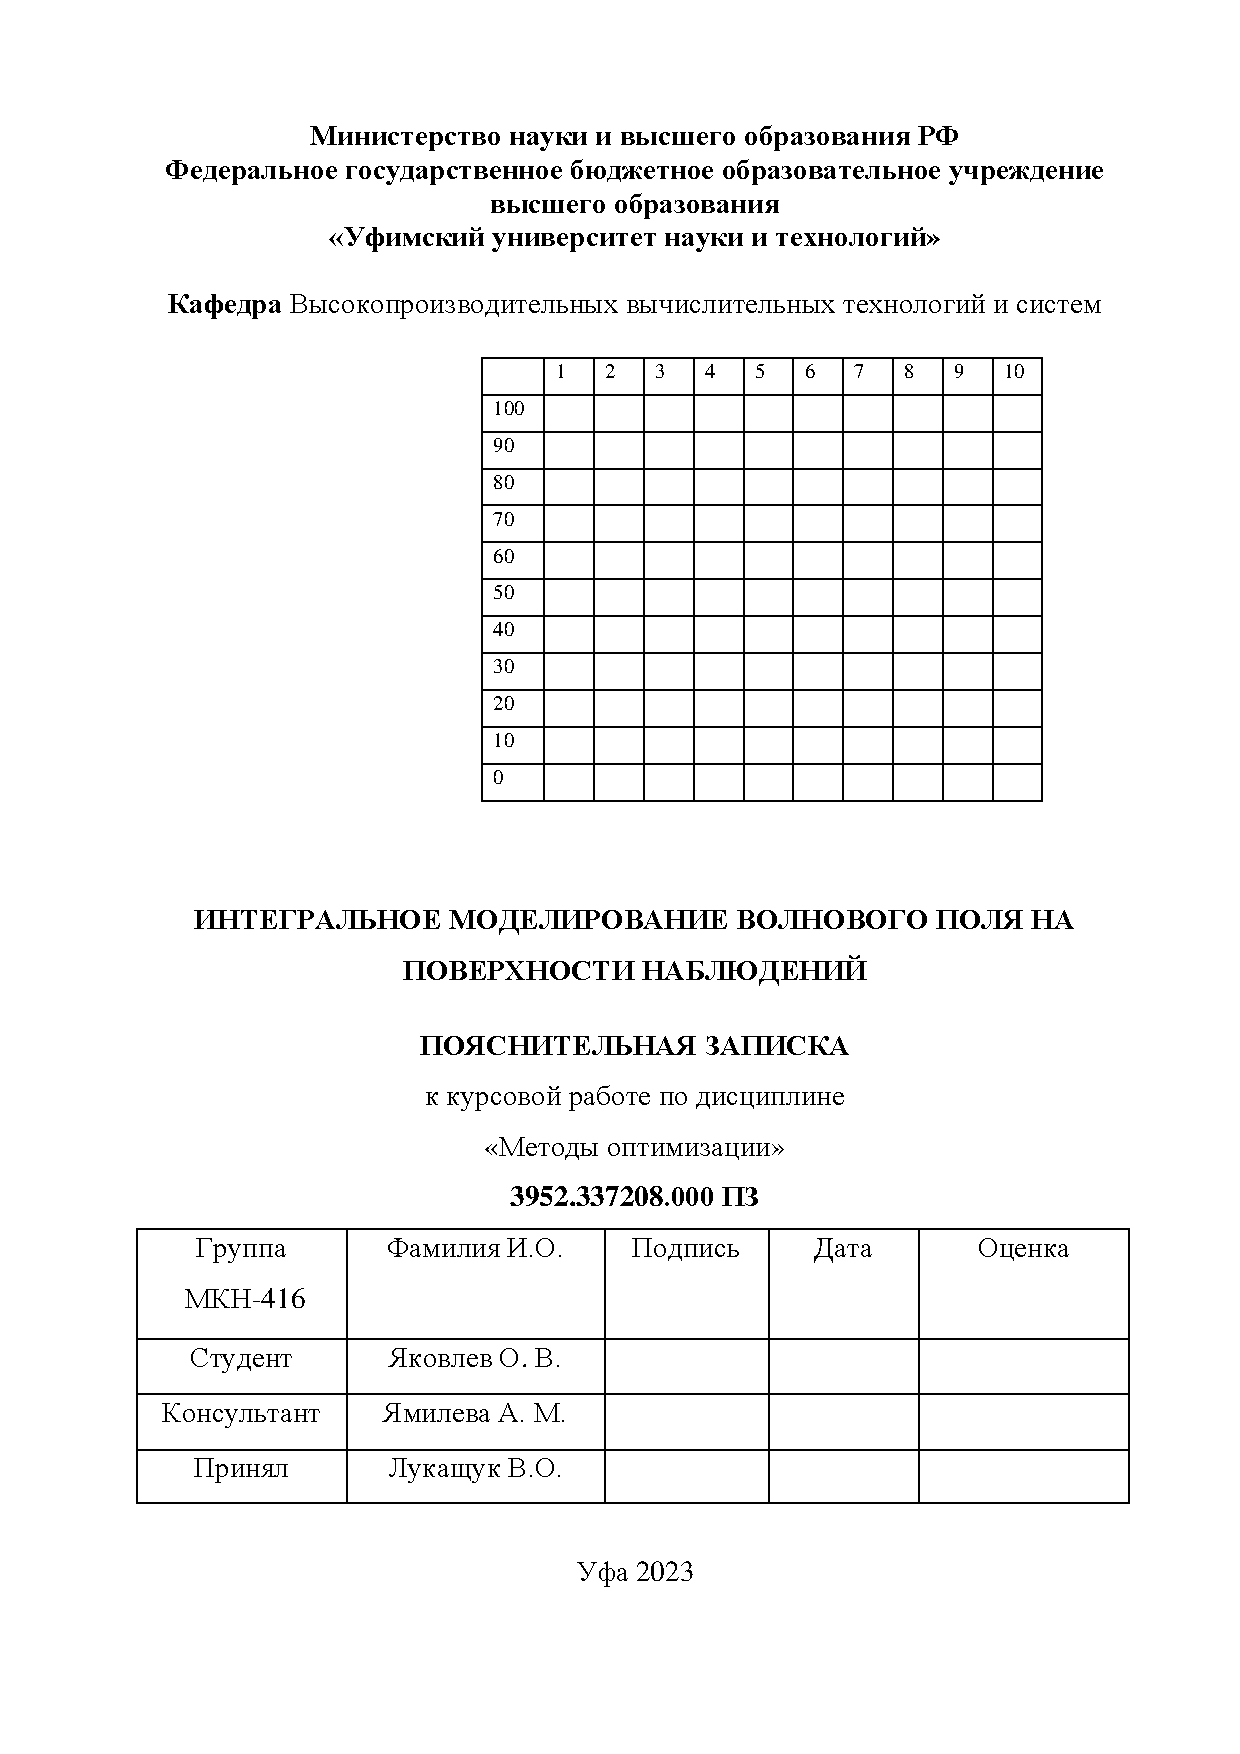
\includepdf[pages=1-3]{cover.pdf}
\newpage
\tableofcontents
\newpage
\section*{Введение}
\addcontentsline{toc}{section}{Введение}

Существует целый класс задач (колебания струны,
движение сжимаемого газа, распространение возмущения электромагнитных полей и многие другие), которые
описываются гиперболическими дифференциальными уравнениями или системами уравнений.
Решение таких уравнений в аналитическом виде
затруднительно, поэтому их зачастую решают численно.
Нередко, из-за трудности получения точного решения, можно прибегнуть к приближенным асимптотическим
методам решения, таким как, например, метод Вентцеля-Крамерса-Бриллюэна (метод ВКБ).
В частности, подобные задачи возникают при моделировании
распространения акустических волн при геолого- и сейсморазведке, где необходимо учесть
и неоднородность среды с учетом эффектов отражения волн от границ слоев с различной плотностью.

Однако, численное решение волнового уравнения может быть
вычислительно затратным. Используя метод интегрального моделирования волнового поля при помощи
демиграции Кирхгофа, можно свести
данную задачу к вычислению интеграла Кирхгофа для каждой точки среды. Такая формулировка задачи
позволяет проводить параллельные вычисления значения волнового поля для каждого момента времени. 
Также демиграция позволяет использовать коэффициенты отражения, получаемые при помощи акустического
каротажа, в качестве входного параметра моделирования.
Акустический каротаж -- это метод геофизического исследования скважин, который применяется для
детального изучения  распределения скорости сейсмических волн вдоль ствола скважин и для определения
вещественного состава и пористости горных пород.
С помощью сейсмического моделирования
наблюдаемого волнового поля можно строить искусственные графики зависимости уровня сигнала 
сейсмических волн или шума от времени их регистрации, называемые сейсмотрассами.

Целью данной курсовой работы является изучение моделирования распространения акустических волн в неоднородной
среде при помощи демиграции по Кирхгофу.
Для достижения данной цели поставлены следующие задачи:
\begin{enumerate}
    \item 
    \item
    \item 
\end{enumerate}
\newpage
\section{Постановка задачи}
Пусть задана область плоскости $D=[0,X]\times[0,Z]$, $z>0$, в пределах которой задано скалярное волновое поле $U(x,z,t)\in\mathbb{R}$, для которого справедливо уравнение \ref{pde}.
 
\begin{equation}
	\label{pde}
	\frac{\partial^2 U(x,z,t)}{\partial x^2} + \frac{\partial^2 U(x,z,t)}{\partial z^2} -  \frac{1}{c^2}\frac{\partial^2 U(x,z,t)}{\partial t^2} = f(x,z,t)
\end{equation}
Задачей является получение аналитической связи
между поверхностным воздействием $f$ и значением волнового поля в произвольной точке рассматриваемой области.


% TODO написать вывод интеграла кирхгофа
Пусть область ограничена и имеет кусочно-гладкую границу $S$.
Тогда по теореме Остроградского-Гаусса можно выразить решение в виде
\begin{equation}
	K(\xi,t) = \frac{1}{2\pi}\int_{z=\Sigma(x)}W(\xi,x,z)  F(t-\tau(\xi,x))\,dS
\end{equation}
\begin{itemize}
	\item $K(\xi,t)$ -- смоделированные сейсмические данные 
	\item $W(\xi,x,z)$ -- весовая функция, состоящая из кажущегося коэффициента отражения прямой волны, падающей на отражатель, и двух амплитуд функций Грина для волны распространяющейся от источника $S$ до $P$, и от $P$ до приемника $G$
				\item $\tau(\xi,x) = T(S(\xi), P(x)) + T(G(\xi), P(x))$ -- сумма времени прохождения волны от
	источника $S$ до точки отражения $P$ и от $P$ до приемника $G$.
	\item $F(t)$ -- импульс источника колебаний.
	\item $\Sigma(x)$ -- отражающая поверхность, вдоль которой идет интегрирование.
\end{itemize}

	Весовую функцию $W(\xi,x,z)$ можно аппроксимировать при помощи функций Грина.
	\begin{equation*}
		\label{demG}
		d(x_s,x_t,t) = \int \int m(x,z) F(t) * G(x_r,0,t|x,z) * \ddot{G}(x,z,t|x_s,0) \,dx\,dz
	\end{equation*}
	
	\begin{itemize}
		\item $G(x_r,0,t|x,z)$ -- Функция Грина волны, распространяющейся от точки отражения $(x,z)$
		до приемника в точке $(x_r,0)$
		\item $G(x,z,t|x_s,0)$ -- Функция Грина волны, распространяющейся от источника $(x_s,0)$
		до точки отражения $(x,z)$
		\item m(x,z) -- Значение миграционного разреза в точке $(x,z)$.
	\end{itemize}
		Функции Грина можно аппроксимировать по методу ВКБ, как
	\begin{gather}
		\label{green1}
		G(x_r,0,t|x,z) = A_{sx} \delta(t - \tau_{x_s0xz}), \\
		\label{green2}
		G(x,z,t|x_s,0) = A_{xr} \delta(t - \tau_{xzx_r0}),
	\end{gather}
	\begin{itemize}
		\item 	$A_{sx}$ и $A_{xr}$ являются амплитудными коэффициентами
		\item 	$\tau_{x_s0xz}$ и $\tau_{xzx_r0}$ -- время распространения колебаний от источника до точки отражения и от точки отражения до приемника соответственно.
	\end{itemize}
	Для среды с постоянной скоростью распространения колебаний $\tau_{x_s0xz}$ и $\tau_{xzx_r0}$ можно вычислить аналитически по формулам
	\begin{gather}
		\tau_{x_s0xz} = \sqrt{\frac{(x_s - x)^2}{V^2} + \frac{z^2}{V^2}} \\
		\tau_{xzx_r0} = \sqrt{\frac{(x_r - x)^2}{V^2} + \frac{z^2}{V^2}}
	\end{gather}
	Поставим в уравнение демиграции \ref{demG} приближения функций Грина \ref{green1} и \ref{green2}.
	\begin{equation}
		d(x_s,x_r,t) = \int \int m(x,z) A_{sx} A_{xr} \ddot{W}(t- \tau_{x_s0xz} -\tau_{xzx_r0} )\,dx\,dz.
	\end{equation}
	



\clearpage


\section*{Заключение}
\addcontentsline{toc}{section}{Заключение}
В ходе выполнения курсовой работы была изучена литература об интегральном моделировании волнового
поля на поверхности наблюдений. Было рассмотрено уравнение Гельмгольца для скалярного волнового
поля и его связь с интегралом Кирхгофа. Было выведено выражение для оператора демграции для
двухмерного пространства и рассмотрено приближение функций Грина для уравнения Гельмгольца по методу
ВКБ. Также был рассмотрен переход от интегральной формы оператора к матричной форме для
упрощения численной реализации.

Была выполнена численная программная реализация интегрального моделирования скалярного волнового
поля при помощи оператора демиграции Кирхгофа. Было смоделировано распространение звуковых волн от
источников, находящихся на поверхности, в слоисто-неоднородной среде. В результате вычислительного 
эксперимента было продемонстрировано отражение волн от границ между слоями среды, и оценена
амплитуда отраженных волн: $A_1 = 600, A_2 = 200, A_3 = 200$.

\newpage

\addcontentsline{toc}{section}{Список литературы}

\printbibliography

\newpage

\includepdf[pages=11]{cover.pdf}

\end{document}
